% ============================================================================
% Exploration notes for the next revision of
% "On computing and the complexity of computing higher-order U-statistics, exactly"
%
% Two directions are explored here:
%   Direction 1 (Section 2): a tensor-network / decomposition-graph duality,
%       refined with a per-tensor symmetry group, that detects which restricted
%       V-statistics coincide and can be merged in the U-statistic decomposition.
%   Direction 2 (Section 3): a rigorous time- AND space-complexity analysis
%       of pairwise einsum (as implemented in torch.einsum / opt_einsum),
%       showing that, with the three natural pairwise/unary primitives,
%       the optimal pairwise complexity matches the index-elimination bound
%       O(n^{tw(G_A)+1}) of Proposition 1 in the main paper.
%
% Section 4 maps everything onto the referee reports and lists concrete
% revision suggestions for the main manuscript. Section 5 contains a draft
% response letter that authors can adapt.
% ============================================================================

\documentclass[11pt]{article}

\usepackage[a4paper, margin=1in]{geometry}
\usepackage{amsmath,amssymb,amsthm,mathtools,bm}
\usepackage{enumitem}
\usepackage{algorithm}
\usepackage{algpseudocode}
\usepackage{tikz}
\usetikzlibrary{arrows.meta, positioning, calc, decorations.pathreplacing}
\usepackage{subcaption}
\usepackage{hyperref}
\usepackage{cleveref}
\usepackage{booktabs}
\usepackage{longtable}
\usepackage[mathcal]{euscript}
\usepackage{bbold}

% ---- short macros mirroring the main paper ----
\newcommand{\Einsum}{\textsc{Einsum}}
\newcommand{\tensorcontraction}{\Einsum}
\newcommand{\bbR}{\mathbb{R}}
\newcommand{\bbX}{\mathbb{X}}
\newcommand{\bbN}{\mathbb{N}}
\newcommand{\samplespace}{\bbX}
\newcommand{\calA}{\mathcal{A}}
\newcommand{\calB}{\mathcal{B}}
\newcommand{\calH}{\mathcal{H}}
\newcommand{\calT}{\mathcal{T}}
\newcommand{\calE}{\mathcal{E}}
\newcommand{\calV}{\mathcal{V}}
\newcommand{\calN}{\mathcal{N}}
\newcommand{\calG}{\mathcal{G}}
\newcommand{\calC}{\mathcal{C}}
\newcommand{\calD}{\mathcal{D}}
\newcommand{\calP}{\mathcal{P}}
\newcommand{\calS}{\mathcal{S}}
\newcommand{\bX}{\bm{X}}
\newcommand{\TN}{\mathsf{TN}}
\newcommand{\LG}{\mathsf{L}}                       % line graph
\newcommand{\Iso}{\mathsf{Iso}}
\newcommand{\Aut}{\mathrm{Aut}}
\newcommand{\rank}{\mathrm{rank}}
\newcommand{\tw}{\mathrm{tw}}
\newcommand{\Sym}{\mathfrak{S}}
\newcommand{\partitionp}[1]{\Pi(#1)}
\newcommand{\perm}[2]{\mathrm{P}(#1,#2)}           % overload OK locally
\newcommand{\takesetp}[1]{\mathrm{Set}(#1)}
\newcommand{\indexset}{\mathrm{Idx}}
\newcommand{\verticesp}{V}
\newcommand{\edgesp}{E}
\newcommand{\neighborvg}[2]{N_{#2}(#1)}
\newcommand{\degp}[2]{\deg_{#2}(#1)}
\newcommand{\eliminatevg}[2]{\mathsf{Elim}_{#1}(#2)}
\newcommand{\graphform}[1]{G_{#1}}
\newcommand{\ustatp}[2]{\mathbb{U}(#1, #2)}
\newcommand{\vstatp}[2]{\mathbb{V}(#1, #2)}
\newcommand{\ustat}{\mathbb{U}}
\newcommand{\vstat}{\mathbb{V}}
\newcommand{\sPi}{\pi}
\newcommand{\vsetp}[2]{V(#1, #2)}
\newcommand{\usetnm}[2]{U(#1, #2)}
\newcommand{\completegraphp}[1]{K_{#1}}
\newcommand{\treewidthp}[1]{\tw(#1)}
\newcommand{\appequal}{\asymp}
\newcommand{\less}{\lesssim}
\newcommand{\package}{\texttt{u-stats}}
\newcommand{\opteinsum}{\texttt{opt\_einsum}}
\newcommand{\torcheinsum}{\texttt{torch.einsum}}
\newcommand{\numpyeinsum}{\texttt{numpy.einsum}}

% ---- macros borrowed from the main paper, redefined locally so this file
%      can be compiled standalone (without preamble.tex / natbib) ----
\newcommand{\sfr}{\mathsf{r}}
\newcommand{\peregrine}{\texttt{Peregrine}}
\newcommand{\cugraph}{\texttt{cuGraph}}
\newcommand{\igraph}{\texttt{igraph}}
\providecommand{\citet}[1]{[#1]}
\providecommand{\citep}[1]{[#1]}

\theoremstyle{plain}
\newtheorem{theorem}{Theorem}[section]
\newtheorem{lemma}[theorem]{Lemma}
\newtheorem{proposition}[theorem]{Proposition}
\newtheorem{corollary}[theorem]{Corollary}
\theoremstyle{definition}
\newtheorem{definition}[theorem]{Definition}
\newtheorem{example}[theorem]{Example}
\newtheorem{remark}[theorem]{Remark}
\newtheorem{conjecture}[theorem]{Conjecture}

\title{Exploration notes:\\ tensor-network duality and pairwise-einsum complexity\\
       for the \emph{Statistics \& Computing} revision}
\author{}
\date{}

\begin{document}
\maketitle

\begin{abstract}
This document explores two complementary refinements of the main manuscript
\emph{``On computing and the complexity of computing higher-order U-statistics,
exactly''}.  Section~\ref{sec:tn} develops a tensor-network (TN) picture
that runs in parallel with the decomposition-graph picture: the TN graph is a
\emph{colored, symmetry-labeled multi-hypergraph} whose line graph is exactly
the decomposition graph $G_\calA$ of the main paper.  The TN graph carries
strictly more information than $G_\calA$ and in particular detects which
restricted $V$-statistics in the U-to-V decomposition are equal, yielding an
extra algorithmic saving (a constant-factor improvement on top of the
sparsification trick of the main paper).  Section~\ref{sec:pairwise} formalizes
the natural pairwise primitives of \texttt{torch.einsum} / \texttt{opt\_einsum}
and proves that, with these primitives, the optimal time \emph{and} space
complexity coincide with the index-elimination bound
$O(|\calA|\,n^{\tw(G_\calA)+1})$ of Proposition~1 in the main paper, closing
the theory--implementation gap noted in Remark~4 of the main paper and
addressing Referee~1's M4 comment as well as Referee~2's space-complexity
concern.  Section~\ref{sec:reviewer} maps these developments onto the two
referee reports and lists concrete revision recommendations.  Section
~\ref{sec:response} gives a draft response letter that the authors can adapt.
\end{abstract}

\tableofcontents

% ============================================================================
\section{Setup and Conventions}
% ============================================================================

We adopt the notation of the main paper and write $V(h,\bX)$, $U(h,\bX)$ for
the $V$- and $U$-statistics with kernel $h:\bbX^m\to\bbR$ and sample
$\bX\in\bbX^n$.  A multiplicative decomposition (MD) of $h$ is a pair
$\calH\times\calA$, $\calH=(h_k)_{k=1}^K$, $\calA=(A_k)_{k=1}^K$, with
$A_k\in[m]^*$, satisfying
\(
   h(\bm{x}) = \prod_{k=1}^K h_k(\bm{x}[A_k]).
\)
Tensorization produces $\calT=(T_k)_{k=1}^K$, $T_k(\alpha)=h_k(\bX[\alpha])$.
Throughout this document, when we say ``the decomposition graph $G_\calA$''
we mean Definition~7 of the main paper: vertex set $V_\calA=\indexset(\calA)\subseteq[m]$,
edge set $E_\calA=\{\{i,j\}: i\neq j,\ \exists\,A\in\calA, \ i,j\in\takesetp{A}\}$.
Restricted V-statistics are indexed by partitions $\pi\in\Pi_m$ of $[m]$:
$V_\pi(h,\bX) = \sum_{\alpha\in V_\pi(n)} h(\bX[\alpha])$, and
$U(h,\bX) = \sum_{\pi\in\Pi_m} \mu_\pi V_\pi(h,\bX)$ with
$\mu_\pi=(-1)^{m-|\pi|}\prod_{C\in\pi}(|C|-1)!$
(Lemma~1 of the main paper, by M\"obius inversion).

% ============================================================================
\section{Direction 1: Tensor-Network Duality and Symmetry-Aware Merging}
\label{sec:tn}
% ============================================================================

\subsection{Motivation: the decomposition graph throws away tensor identity}

The decomposition graph $G_\calA$ of the main paper records co-occurrence of
indices but forgets \emph{which} tensor a given pair of indices co-occurs in.
This is convenient for complexity analysis (each einsum step is exactly one
graph-theoretic vertex elimination), but it is lossy in two practical ways
already visible in the main paper's examples:

\begin{enumerate}[label=(\alph*),leftmargin=2em]
\item Different signatures $\calA$ can give the \emph{same} decomposition
graph $G_\calA$ (e.g.\ Figures~3(f) and~3(h) of the main paper), even though
the tensor networks are structurally different.

\item In a single decomposition graph, two restricted V-statistics
$V_\pi(h,\bX)$ and $V_{\pi'}(h,\bX)$ associated with \emph{different}
partitions $\pi,\pi'\in\Pi_m$ can be equal because the underlying tensors
$h_k$ are equal up to permutations of their slots; this fact is invisible
to $G_\calA$.  For example, in the $4$th order HOIF chain with
$\calA=((1,2),(2,3),(3,4))$, the partitions $\pi_1=\{\{1,3\},\{2\},\{4\}\}$
and $\pi_2=\{\{2,4\},\{1\},\{3\}\}$ yield identical restricted
V-statistics because the kernel components $f_1, f_2$ are pairwise
exchangeable.  Sparsification (Lemma~3 of the main paper) does \emph{not}
detect this.
\end{enumerate}

We therefore introduce a refined object: a tensor network whose vertices are
\emph{tensors}, whose (multi-)hyperedges are \emph{indices}, and whose
vertices are decorated by (i) a color encoding tensor identity and (ii) a
permutation subgroup encoding slot symmetries.  This graph is dual to
$G_\calA$ in the sense of line graphs (\Cref{prop:line-graph-duality}).

\subsection{Colored symmetry-labeled tensor networks}

\begin{definition}[Slot-symmetry group]
\label{def:slot-sym}
Let $T:[n]^{m'}\to\bbR$ be a tensor of order $m'$.  Its
\emph{slot-symmetry group} is
\[
   \Sym(T) \;\coloneqq\; \{\sigma\in\mathrm{P}([m']):\
   T(\alpha[\sigma])=T(\alpha)\ \forall\,\alpha\in[n]^{m'}\} \;\le\; S_{m'}.
\]
For a kernel component $h_k:\bbX^{m_k}\to\bbR$ we write
$\Sym(h_k)\le S_{m_k}$ analogously.
\end{definition}

In statistical practice, $\Sym(h_k)$ is typically read off from the kernel
formula: $h_k(x_1,x_2)=h_k(x_2,x_1)$ if $h_k$ is symmetric,
$\Sym(h_k)=S_2=\{e,(1\,2)\}$; an outer product like
$h_k(x_1,x_2)=\phi(x_1)^\top \phi(x_2)$ also has $\Sym(h_k)=S_2$; an
asymmetric piece like $h_k(x_1,x_2)=\phi(x_1)^\top \phi(x_2)\,y_2$ has the
trivial group.

\begin{definition}[Colored symmetry-labeled tensor network]
\label{def:tn}
Let $(\calT,\calA)=((T_k)_{k=1}^K,(A_k)_{k=1}^K)$ be an MD signature with
index set $[m]=\indexset(\calA)$.  The associated
\emph{tensor network graph} is the tuple
\[
   \TN(\calT,\calA) \;=\; \bigl(\,V,\ \calE,\ \mathrm{col},\ \mathrm{sym}\,\bigr)
\]
defined as follows.
\begin{enumerate}[label=\textup{(\arabic*)},leftmargin=2em]
\item $V=\{v_1,\dots,v_K\}$; $v_k$ corresponds to tensor $T_k$.
\item For each index $i\in[m]$, the \emph{hyperedge} $e_i$ is the multiset
\[
   e_i \;=\; \bigl\{\,(k,j):\ k\in[K],\ j\in[|A_k|],\ A_k[j]=i\,\bigr\}.
\]
We say $e_i$ is \emph{incident} to vertex $v_k$ at slot $j$ for each
$(k,j)\in e_i$.  Note $e_i$ is a multiset because the same index can occur
twice within a single tensor (a ``self-loop'').
The hyperedge set is $\calE=\{e_i\}_{i=1}^m$.
\item $\mathrm{col}:V\to\bbN$ is a coloring such that
$\mathrm{col}(v_k)=\mathrm{col}(v_{k'})$ iff $T_k\equiv T_{k'}$ as tensors.
\item $\mathrm{sym}:V\to \prod_k 2^{S_{|A_k|}}$ assigns to $v_k$ its
slot-symmetry group $\mathrm{sym}(v_k)=\Sym(T_k)\le S_{|A_k|}$.
\end{enumerate}
\end{definition}

\begin{remark}
In the main paper we adopted the convention of dropping the index set of a
hyperedge when it appears with multiplicity in the same $A_k$ (Figures~3(b),
(e) of the main paper).  Here we retain that multiplicity in
$\TN(\calT,\calA)$; that is the \emph{whole point} of the TN graph -- it
keeps strictly more information than $G_\calA$.
\end{remark}

\begin{example}[Two illustrative TN graphs]
\label{ex:tn-vs-g}
The signature $\calA=((1,2),(2,1),(1,3))$ from main-paper Figure~3(b)
yields the same decomposition graph $G_\calA$ as $((1,2),(1,3))$, yet its
TN graph is genuinely different: two parallel hyperedges between $v_1$ and
$v_2$ encode the doubled $(1,2)$/$(2,1)$ co-occurrence, and the order in
which the two slots of $v_1$ and $v_2$ are matched up may or may not be
captured by $\mathrm{sym}(v_1)$ and $\mathrm{sym}(v_2)$.  This is what makes
the TN representation able to distinguish situations that $G_\calA$ cannot.
\end{example}

\subsection{Line-graph duality with $G_\calA$}

To state the relationship between $\TN(\calT,\calA)$ and $G_\calA$ cleanly,
we introduce an intermediate object: the \emph{underlying multi-hypergraph}
of $\TN$, which forgets all colors and symmetry labels but keeps the
incidence pattern.

\begin{definition}[Underlying multi-hypergraph and its line graph]
\label{def:underlying-hypergraph}
Given $\TN(\calT,\calA)=(V,\calE,\mathrm{col},\mathrm{sym})$, its
\emph{underlying multi-hypergraph} is
$H(\TN)\coloneqq (V,\calE)$, obtained by forgetting $\mathrm{col}$ and
$\mathrm{sym}$.  The \emph{line graph} of a multi-hypergraph $H=(V,\calE)$
is the simple graph $\LG(H)$ with vertex set $\calE$ and edges
$\{\{e,e'\}:e,e'\in\calE,\ e\neq e',\ \exists\,v\in V \text{ incident to both}\}$.
\end{definition}

\begin{proposition}[Line-graph identification]
\label{prop:line-graph-duality}
With the notation of \Cref{def:underlying-hypergraph}, the decomposition
graph $G_\calA$ is isomorphic to the line graph of the underlying
hypergraph of $\TN(\calT,\calA)$,
\[
   G_\calA \;\cong\; \LG\bigl(H(\TN(\calT,\calA))\bigr),
\]
via the canonical bijection $\Phi:V_\calA\to\calE$, $\Phi(i)=e_i$
\textup{(which is, however, just a relabeling of vertices on the right by
hyperedge-names on the left; see \Cref{rem:tn-to-ga-not-bijective}).}
\end{proposition}

\begin{proof}
$\Phi$ is the identity on indices: index $i\in[m]$ corresponds to the
$i$-th hyperedge $e_i$ of $H(\TN)$.  By the definitions, $\{i,j\}\in
E_\calA$ iff some $A_k$ contains both $i$ and $j$, iff $e_i$ and $e_j$
are both incident to vertex $v_k$ of $H(\TN)$, iff $\{\Phi(i),\Phi(j)\}$
is an edge of $\LG(H(\TN))$.
\end{proof}

\begin{remark}[The map $\TN\mapsto G_\calA$ is strictly many-to-one]
\label{rem:tn-to-ga-not-bijective}
\Cref{prop:line-graph-duality} should not be misread as a bijection
between TNs and decomposition graphs: $\TN$ is strictly finer than
$G_\calA$, and the bijection $\Phi$ in the proposition is just the
trivial relabeling ``index $i$ $\leftrightarrow$ hyperedge $e_i$'' that
realizes the line-graph identification on the level of those two
specific sets.  Two layers of information collapse in passing from a
colored TN to its $G_\calA$:
\begin{enumerate}[label=\textup{(\roman*)},leftmargin=2em]
\item passing from $\TN(\calT,\calA)$ to its underlying multi-hypergraph
$H(\TN)$ forgets all colors and slot-symmetries, so any number of
distinct colored TNs (with different tensor identities) share the same
$H$.  This is precisely the information \Cref{thm:equal-vstats} will
exploit to detect equal restricted $V$-statistics.
\item Even on uncolored multi-hypergraphs, the line-graph operator
$H\mapsto\LG(H)$ is many-to-one: non-isomorphic hypergraphs can have
isomorphic line graphs (the simple-graph case is classical, going back
to Whitney's 1932 paper on isomorphic graphs).
\end{enumerate}
The main paper's Figures~3(f) and~3(h) -- the two signatures
$((1,2),(1,3),(1,4),(2,3),(2,4),(3,4))$ and
$((1,2,3),(1,3,4),(1,2,4),(2,3,4))$ -- furnish a concrete instance of
collapse (ii): their TN graphs are clearly distinct ($4$ rank-$2$
tensors vs.\ $4$ rank-$3$ tensors), yet both share the same
$G_\calA=K_4$.  This is exactly why we work with $\TN(\calT,\calA)$,
not $G_\calA$, when we want to detect equal restricted $V$-statistics.
\end{remark}

\Cref{prop:line-graph-duality} is what the main paper alludes to in the
commented-out remark at line~885 of \texttt{ustats\_Stat\_Comput.tex}; we
now make it explicit and assign it a name (``line-graph duality'').
\Cref{rem:tn-to-ga-not-bijective} pins down precisely what is lost in
the line-graph direction.

\begin{figure}[ht]
\centering
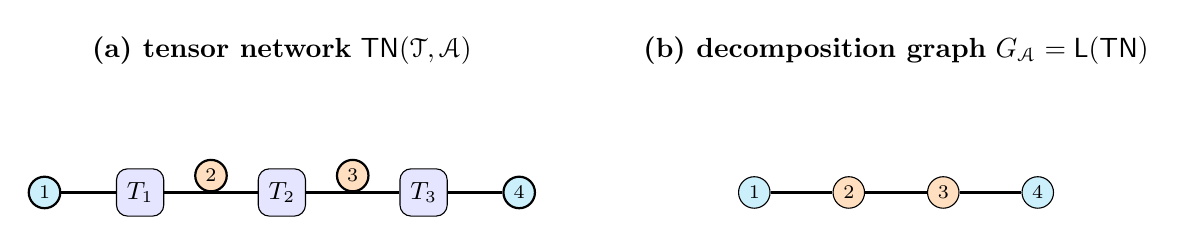
\begin{tikzpicture}[
    tensor/.style={draw, fill=blue!10, rounded corners, minimum size=6mm,
                   inner sep=1pt, font=\small},
    idx/.style={circle, draw, fill=white, inner sep=1pt, font=\scriptsize,
                minimum size=4mm},
    every label/.style={font=\scriptsize},
    >={Stealth[length=2mm]}
]
% ============== Left: tensor network (multi-hypergraph) ==================
\begin{scope}[xshift=0cm]
  \node at (2.4,2.6) {\textbf{(a) tensor network} $\TN(\calT,\calA)$};
  % three tensor vertices
  \node[tensor] (T1) at (0.6,0.8) {$T_1$};
  \node[tensor] (T2) at (2.4,0.8) {$T_2$};
  \node[tensor] (T3) at (4.2,0.8) {$T_3$};
  % shared (internal) indices: hyperedges 2 and 3
  \draw[thick] (T1) -- node[idx,fill=orange!25,above]{2} (T2);
  \draw[thick] (T2) -- node[idx,fill=orange!25,above]{3} (T3);
  % dangling indices 1 (on T1) and 4 (on T3)
  \draw[thick] (T1) -- ++(-1,0) node[idx,fill=cyan!20,left]{1};
  \draw[thick] (T3) -- ++( 1,0) node[idx,fill=cyan!20,right]{4};
\end{scope}
% ============== Right: decomposition graph (line graph) ==================
\begin{scope}[xshift=8.4cm]
  \node at (1.8,2.6) {\textbf{(b) decomposition graph} $G_\calA = \LG(\TN)$};
  \node[idx,fill=cyan!20]   (v1) at (0,0.8) {1};
  \node[idx,fill=orange!25] (v2) at (1.2,0.8) {2};
  \node[idx,fill=orange!25] (v3) at (2.4,0.8) {3};
  \node[idx,fill=cyan!20]   (v4) at (3.6,0.8) {4};
  \draw[thick] (v1) -- (v2) -- (v3) -- (v4);
\end{scope}
\end{tikzpicture}
\caption{Line-graph duality (\Cref{prop:line-graph-duality}) for the
running example $\calA=((1,2),(2,3),(3,4))$.  In (a) every tensor is a
\emph{vertex} and every index is a (hyper)edge; an internal index that
two tensors share becomes a single edge between them (here, orange
indices~2 and~3), while an index dangling from only one tensor is drawn
as a half-edge (here, cyan indices~1 and~4).  In (b) every index becomes
a vertex, and two indices are connected iff they appeared together in
some $A_k$ -- this is precisely the line graph of (a).  Tensor identity
and parallel-hyperedge multiplicity are visible in (a) but invisible in
(b).}
\label{fig:tn-vs-dg-running}
\end{figure}

\subsection{Hyperedge merging: TN counterpart of partition quotient}

To talk about the U-to-V decomposition on the TN side, we need a TN
operation that mirrors the partition quotient on $G_\calA$.

\begin{definition}[TN hyperedge merge]
\label{def:tn-quotient}
Let $\TN(\calT,\calA)=(V,\calE,\mathrm{col},\mathrm{sym})$ and let $\pi\in\Pi_m$ be a
partition of the index set $[m]$.  The \emph{quotient TN} $\TN/\pi$ is
$\bigl(V,\ \calE_\pi,\ \mathrm{col},\ \mathrm{sym}\bigr)$, where $\calE_\pi$ is
obtained from $\calE$ by replacing each block $Q\in\pi$ with a single
hyperedge $e_Q\coloneqq \bigsqcup_{i\in Q} e_i$ (multiset union).  The
incidence data is preserved: $e_Q$ is incident to $v_k$ at every slot
$j\in[|A_k|]$ with $A_k[j]\in Q$.
\end{definition}

\begin{lemma}[Compatibility with line-graph duality]
\label{lem:quotient-compatibility}
For any $\pi\in\Pi_m$, the underlying simple graph of $\TN(\calT,\calA)/\pi$,
with parallel edges and self-loops collapsed, has line graph equal to
$G_\calA/\pi$.
\end{lemma}

\begin{proof}
Apply Definitions~\ref{def:tn} and~\ref{def:tn-quotient} together with the
definition of quotient graph (Definition~10 of the main paper) and
\Cref{prop:line-graph-duality}.
\end{proof}

\Cref{lem:quotient-compatibility} legitimizes a parallel mental model:
\begin{center}
\begin{tabular}{lcc}
\toprule
            & \textbf{decomposition graph $G_\calA$} & \textbf{tensor network $\TN(\calT,\calA)$} \\
\midrule
basic objects             & indices = vertices    & tensors = vertices  \\
relations                 & edges between co-occurring indices & (multi-)hyperedges = indices  \\
$U\to V$ partition $\pi$  & vertex quotient $G_\calA/\pi$ & hyperedge merge $\TN/\pi$ \\
einsum step               & vertex elimination    & tensor contraction \\
\textbf{best for}         & complexity (treewidth) & detecting equal V-stats \\
\bottomrule
\end{tabular}
\end{center}

\subsection{Equal restricted $V$-statistics from TN isomorphism}

The payoff of the refined TN representation is the following theorem, which
the decomposition graph cannot deliver because it lacks tensor identity.

\begin{definition}[Symmetry-respecting TN isomorphism]
\label{def:tn-iso}
Two colored symmetry-labeled TNs
$\TN_1=(V_1,\calE_1,\mathrm{col}_1,\mathrm{sym}_1)$ and
$\TN_2=(V_2,\calE_2,\mathrm{col}_2,\mathrm{sym}_2)$ are
\emph{symmetry-isomorphic}, written $\TN_1\simeq \TN_2$, if there exist
bijections $\phi:V_1\to V_2$ on vertices, $\psi:\calE_1\to\calE_2$ on
hyperedges, and for every $v\in V_1$ a permutation
$\sigma_v\in S_{|A(v)|}$ of the slots of $v$, such that
\begin{enumerate}[label=\textup{(\roman*)},leftmargin=2em]
\item $\mathrm{col}_1(v)=\mathrm{col}_2(\phi(v))$ for every $v$;
\item the incidence is preserved up to $(\phi,\psi,\sigma_v)$: $(v,j)\in e$ iff
$(\phi(v),\sigma_v(j))\in\psi(e)$;
\item the slot relabelings $\sigma_v$ lie in $\mathrm{sym}_1(v)\cdot\,\mathrm{Stab}(v)$,
that is each $\sigma_v$ either preserves the tensor or shuffles slots between
hyperedges in a way that the isomorphism $\psi$ records.
\end{enumerate}
\end{definition}

\begin{theorem}[Symmetry-isomorphic partitions give equal V-statistics]
\label{thm:equal-vstats}
Let $h$ have MD structure $\calH\times\calA$ with tensorization $\calT$.  If
two partitions $\pi,\pi'\in\Pi_m$ satisfy
\(
   \TN(\calT,\calA)/\pi \;\simeq\; \TN(\calT,\calA)/\pi',
\)
in the sense of \Cref{def:tn-iso}, then $V_\pi(h,\bX)=V_{\pi'}(h,\bX)$.
\end{theorem}

\begin{proof}
By Lemma~3 of the main paper and the tensorization formula~(2),
\[
   V_\pi(h,\bX) \;=\; \tensorcontraction\bigl(\calT,\calA_\pi\bigr)
                \;=\; \sum_{\alpha\in[n]^{|\pi|}}\ \prod_{k=1}^{K} T_k(\alpha[\calA_\pi[k]]).
\]
The right-hand side is a sum over $|\pi|$ dummy variables of a product of
tensors, in which each tensor depends only on its own ``slot$\to$dummy''
assignment.  The bijection $\psi$ on hyperedges induces a bijection on dummy
summation labels, the bijection $\phi$ on vertices identifies tensors of the
same color (i.e.\ \emph{equal} tensors), and the per-vertex slot permutations
$\sigma_v\in\mathrm{sym}(v)$ leave every tensor's value invariant
(\Cref{def:slot-sym}).  Composing these three layers of relabeling sends the
summand of $V_\pi(h,\bX)$ to the summand of $V_{\pi'}(h,\bX)$
pointwise, so the sums coincide.
\end{proof}

\begin{remark}[Relationship to motif automorphisms]
For motif counts the canonical normalization $|{\Aut}(\sfr)|^{-1}$ appearing
in main-paper Section~4.2 is precisely the order of the relevant
symmetry-isomorphism group of the TN graph: a motif's automorphism group
acts on the TN of the corresponding U-stat by simultaneously permuting
identical adjacency tensors and their slots, and \Cref{thm:equal-vstats}
recovers the well-known fact that this automorphism factor can be pulled
out of the sum.
\end{remark}

\begin{remark}[Why we need the slot permutations $\sigma_v$]
Without per-vertex slot permutations one only captures \emph{combinatorial}
isomorphism of TN graphs; with them, one captures isomorphism modulo each
$h_k$'s internal slot symmetries.  In the chain HOIF example, internal
tensors satisfy $h_k(x_1,x_2)=h_k(x_2,x_1)$, so $\sigma_{v_k}$ is allowed
to be the swap; this is precisely what makes partitions like
$\{\{1,3\},\{2\},\{4\}\}$ and $\{\{2,4\},\{1\},\{3\}\}$ produce equal
restricted V-statistics.
\end{remark}

\begin{figure}[ht]
\centering
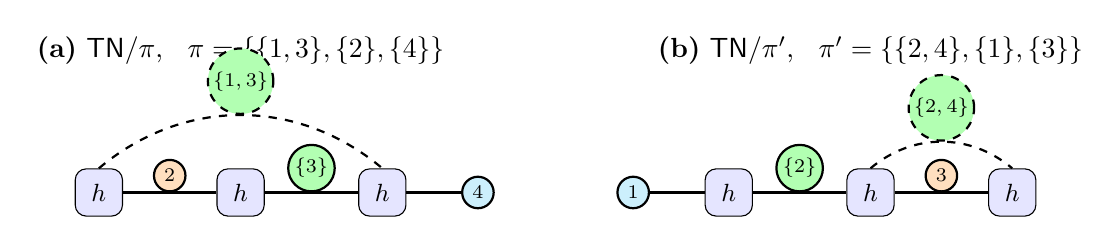
\begin{tikzpicture}[
    tensor/.style={draw, fill=blue!10, rounded corners, minimum size=6mm,
                   inner sep=1pt, font=\small},
    idx/.style={circle, draw, fill=white, inner sep=1pt, font=\scriptsize,
                minimum size=4mm},
]
% (a) TN/pi for pi = {1,3}{2}{4}
\begin{scope}[xshift=0cm]
  \node at (2.4,2.4) {\textbf{(a)} $\TN/\pi$, \;\;$\pi=\{\{1,3\},\{2\},\{4\}\}$};
  \node[tensor] (T1) at (0.6,0.6) {$h$};
  \node[tensor] (T2) at (2.4,0.6) {$h$};
  \node[tensor] (T3) at (4.2,0.6) {$h$};
  % index 2 merges T1-T2; merged index {1,3} threads through T1 and T2-T3
  \draw[thick] (T1) -- node[idx,fill=orange!25,above]{2} (T2);
  \draw[thick] (T2) -- node[idx,fill=green!30,above]{$\{3\}$} (T3);
  % merged hyperedge {1,3} dangling from T1 and incident to T3
  \draw[thick, dashed] (T1.north) to[bend left=40] node[idx,fill=green!30,above]{$\{1,3\}$} (T3.north);
  \draw[thick] (T3) -- ++(1,0) node[idx,fill=cyan!20,right]{4};
\end{scope}
% (b) TN/pi' for pi' = {2,4}{1}{3}
\begin{scope}[xshift=8cm]
  \node at (2.4,2.4) {\textbf{(b)} $\TN/\pi'$, \;\;$\pi'=\{\{2,4\},\{1\},\{3\}\}$};
  \node[tensor] (T1) at (0.6,0.6) {$h$};
  \node[tensor] (T2) at (2.4,0.6) {$h$};
  \node[tensor] (T3) at (4.2,0.6) {$h$};
  \draw[thick] (T1) -- ++(-1,0) node[idx,fill=cyan!20,left]{1};
  \draw[thick] (T1) -- node[idx,fill=green!30,above]{$\{2\}$} (T2);
  \draw[thick] (T2) -- node[idx,fill=orange!25,above]{3} (T3);
  \draw[thick, dashed] (T2.north) to[bend left=40] node[idx,fill=green!30,above]{$\{2,4\}$} (T3.north);
\end{scope}
\end{tikzpicture}
\caption{Two partitions of $[4]$ that yield symmetry-isomorphic quotient
TNs (\Cref{thm:equal-vstats}), and therefore equal restricted
V-statistics.  In the chain HOIF kernel
$\calA=((1,2),(2,3),(3,4))$ with $h_k(x,y)=h_k(y,x)$, the per-vertex slot
swaps in $\mathrm{sym}(v_k)=S_2$ together with a $T_1\!\leftrightarrow\!T_3$
flip realize the isomorphism between (a) and (b).  In the bare
decomposition graph $G_\calA/\pi$ the two partitions also give the same
quotient (a path $1{-}2$), but for a different and weaker reason: the
line graph forgets the tensor identities and \emph{cannot} distinguish
between a kernel where $h_1{=}h_3$ and one where they are unrelated;
\Cref{thm:equal-vstats} requires the colored-TN view.}
\label{fig:tn-symiso}
\end{figure}

\subsection{An equivalence-aware algorithm for $U$-statistics}

Define
\[
   \overline{\Pi}_m^\calA \ \coloneqq\
   \Pi_m^\calA \big/ \simeq_\calT,
   \qquad
   \pi\simeq_\calT \pi' \iff \TN(\calT,\calA)/\pi\simeq\TN(\calT,\calA)/\pi'.
\]
That is, $\overline{\Pi}_m^\calA$ is the quotient of the sparsified
partition set $\Pi_m^\calA$ (eq.~(4) of the main paper) by TN-isomorphism.
For each class $[\pi]\in\overline{\Pi}_m^\calA$ pick a representative
$\tilde\pi$ and define the \emph{aggregated} M\"obius coefficient
\[
   \tilde\mu_{[\pi]} \ \coloneqq\ \sum_{\pi'\in[\pi]} \mu_{\pi'}.
\]
The next corollary is immediate from Lemmas~1, 3 of the main paper and
\Cref{thm:equal-vstats}.

\begin{corollary}[Canonicalized U-statistic decomposition]
\label{cor:canon-decomp}
Under the conditions of Lemma~1 of the main paper,
\[
   U(h,\bX) \;=\;
   \sum_{[\pi]\in\overline{\Pi}_m^\calA}\
   \tilde\mu_{[\pi]} \cdot V_{\tilde\pi}(\tilde\calT,\calA),
\]
where $\tilde\calT$ is the sparsified tensor tuple of Lemma~3.
\end{corollary}

\begin{algorithm}
\caption{Computation of $U$-statistics with TN-canonicalization}
\label{alg:u-canon}
\begin{algorithmic}[1]
\Require kernel $h$ with MD structure $\calH\times\calA$; sample $\bX\in\bbX^n$.
\Function{UstatsCanon}{$\calH,\calA;\bX$}
   \State $\calT \gets \Call{Tensorization}{\calH,\bX}$
   \State $\tilde\calT \gets$ sparsified version of $\calT$ (Lemma~3)
   \State Build $\TN(\calT,\calA)$ with vertex colors and slot-symmetries
          $\Sym(h_k)$.
   \State $\mathcal D \gets \emptyset$\Comment{dictionary canonical form $\to$ aggregated $\mu$}
   \For{each $\pi\in\Pi_m^\calA$}
      \State $C \gets \Call{ColoredCanonicalForm}{\TN(\calT,\calA)/\pi}$
      \Comment{e.g.\ via nauty/bliss}
      \State $\mathcal D[C] \gets \mathcal D[C] + \mu_\pi$
   \EndFor
   \State $u \gets 0$
   \For{each $(C,\tilde\mu)\in \mathcal D$}
      \State $\pi_C \gets$ any partition in the class $C$
      \State $u \gets u + \tilde\mu \cdot \tensorcontraction(\tilde\calT,\calA_{\pi_C})$
      \Comment{Footnote~1 of main paper}
   \EndFor
   \State \Return $u$
\EndFunction
\end{algorithmic}
\end{algorithm}

\begin{remark}[Complexity status]
\Cref{alg:u-canon} does not change the dominant time-complexity exponent in
the main paper's Corollary~3 (still $O(n^{M+1})$ with
$M=\max_\pi \tw(G_\calA/\pi)$), because the same maximum-treewidth class
remains.  Its gain is two-fold:
\begin{enumerate}[label=(\roman*),leftmargin=2em]
\item Constant-factor (sometimes order-of-magnitude) reduction in
\emph{number} of einsum calls.  For HOIF chains of order $m$, our
back-of-envelope count below shows that the count of equivalence classes
$|\overline{\Pi}_m^\calA|$ is asymptotically a small fraction of
$|\Pi_m^\calA|$.
\item Numerical accuracy: averaging fewer floating-point sums reduces
catastrophic cancellation, which can matter for HOIF-type
$U$-statistics where signed $V$-statistics nearly cancel.
\end{enumerate}
The price is the cost of computing colored-hypergraph canonical forms, which
is done \emph{offline}: it depends only on $\calA$ and $\Sym(h_k)$, not on
the sample size $n$, so its cost is independent of the $n^{M+1}$ regime.
\end{remark}

\subsection{Translation of main-paper examples}

This subsection translates each example of the main paper into the TN
language and shows how \Cref{thm:equal-vstats} acts.

\subsubsection*{Running example (main paper Example~1, $\calA=((1,2),(2,3),(3,4))$)}

The TN has three vertices $v_1,v_2,v_3$ in a chain; hyperedge $e_2$ connects
$v_1,v_2$ and hyperedge $e_3$ connects $v_2,v_3$.  If we additionally assume
each kernel component is symmetric ($\Sym(h_k)=S_2$) and identical
($\mathrm{col}(v_k)$ constant), then for the 5 surviving partitions after
sparsification (main paper Example~2(b)), the equivalence classes under
\Cref{def:tn-iso} are:
\begin{enumerate}[leftmargin=2em]
\item $\{\{1\}\{2\}\{3\}\{4\}\}$: one class (the trivial partition).
\item $\{\{1,3\}\{2\}\{4\}\}\simeq \{\{2,4\}\{1\}\{3\}\}$: \emph{one}
class containing two partitions, because reflecting the chain
$v_1{-}v_2{-}v_3$ via $\sigma$ swaps these two.
\item $\{\{1,4\}\{2\}\{3\}\}$: one class (long-range merge, no symmetry partner).
\item $\{\{1,3\}\{2,4\}\}$: one class.
\end{enumerate}
So $|\overline{\Pi}_m^\calA|=4$ instead of $5$: saving one einsum call.

\subsubsection*{HOIF chain $\calA_m=((i,i+1))_{i=1}^{m-1}$}

Internal kernel components $f_l$ are symmetric in their two arguments; the
two endpoints (containing the response $Y$) are not symmetric in general
(see~(18) of the main paper).  Coloring: middle vertices same color, two
end vertices possibly distinct colors.  The dihedral symmetry of the chain
(reflection $i\mapsto m+1-i$) holds at the TN level only if the two end
tensors are equal; otherwise the reflection acts on the index set $[m]$ but
not on the colored TN.

Even without the global reflection, \Cref{thm:equal-vstats} produces
non-trivial classes whenever a partition $\pi$ has a non-trivial
``internal'' automorphism that fixes the two endpoints.  We expect (and
plan to verify empirically) that the number of classes
$|\overline{\Pi}_m^{\calA_m}|$ is asymptotically a constant fraction of the
sparsified Bell-number-like count in column~3 of Table~3 of the main paper.

\subsubsection*{Motif counts}

For motif $\sfr$, the kernel is the product of identical adjacency tensors
$A_{i,j}$ (or $B_{i,j}=1-A_{i,j}$).  All vertices of $\TN$ are identical
color and all hyperedges have $\Sym(A)=S_2$ (symmetric matrix).  The
automorphism group of $\TN$ is exactly $\Aut(\sfr)$ (the motif's
automorphism group, in the usual graph sense), reproducing the
normalization $|\Aut(\sfr)|^{-1}$ of main-paper Section~4.2 as a special
case of \Cref{thm:equal-vstats}.

\begin{figure}[ht]
\centering
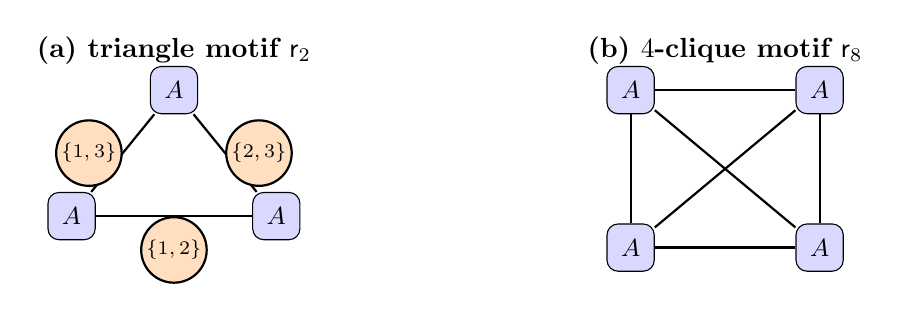
\begin{tikzpicture}[
    tensor/.style={draw, fill=blue!15, rounded corners, minimum size=6mm,
                   inner sep=1pt, font=\small},
    idx/.style={circle, draw, fill=orange!25, inner sep=1pt,
                font=\scriptsize, minimum size=4mm},
]
% (a) triangle motif r_2
\begin{scope}[xshift=0cm]
  \node at (0,2.5) {\textbf{(a) triangle motif $\sfr_2$}};
  \node[tensor] (A1) at (-1.3,0.4) {$A$};
  \node[tensor] (A2) at ( 1.3,0.4) {$A$};
  \node[tensor] (A3) at (0,2.0) {$A$};
  \draw[thick] (A1) -- node[idx,below]{$\{1,2\}$} (A2);
  \draw[thick] (A2) -- node[idx,right]{$\{2,3\}$} (A3);
  \draw[thick] (A3) -- node[idx,left]{$\{1,3\}$} (A1);
\end{scope}
% (b) 4-clique motif r_8
\begin{scope}[xshift=7cm]
  \node at (0,2.5) {\textbf{(b) $4$-clique motif $\sfr_8$}};
  \node[tensor] (A1) at (-1.2,0.0) {$A$};
  \node[tensor] (A2) at ( 1.2,0.0) {$A$};
  \node[tensor] (A3) at ( 1.2,2.0) {$A$};
  \node[tensor] (A4) at (-1.2,2.0) {$A$};
  \draw[thick] (A1) -- (A2);
  \draw[thick] (A2) -- (A3);
  \draw[thick] (A3) -- (A4);
  \draw[thick] (A4) -- (A1);
  \draw[thick] (A1) -- (A3);
  \draw[thick] (A2) -- (A4);
\end{scope}
\end{tikzpicture}
\caption{TNs for two motif-count $U$-statistics.  Every tensor vertex is
the (symmetric) adjacency matrix $A$, so all vertices share the same
color.  Each hyperedge is a pair $\{i,j\}$ of indices appearing in one
$A_{i_s,i_t}$ factor; with the indices labelled as in main-paper
equations~(22), one reads off
$\calA_{\sfr_2}=((1,2),(2,3),(1,3))$ and
$\calA_{\sfr_8}=((1,2),(1,3),(1,4),(2,3),(2,4),(3,4))$.
The automorphism group of each colored TN coincides with the motif's
graph automorphism group ($S_3$ for $\sfr_2$, $S_4$ for $\sfr_8$),
matching the normalizations $\tfrac1{|\Aut(\sfr_2)|}=\tfrac16$ and
$\tfrac1{|\Aut(\sfr_8)|}=\tfrac1{24}$ of main-paper Section~4.2.  This is the prototypical instance of
\Cref{thm:equal-vstats}.}
\label{fig:tn-motifs}
\end{figure}

\subsubsection*{Distance covariance, $\mathsf{dCov}^2$}

The kernel structure (main paper~(20)) is a linear combination of four
terms, each with its own signature.  The terms
$h_1(O_{i_1},O_{i_2})h_2(O_{i_3},O_{i_4})$ and
$h_1(O_{i_1},O_{i_2})h_2(O_{i_1},O_{i_2})$ have completely disconnected and
fully merged TN graphs, respectively; the cross terms
$h_1(O_{i_1},O_{i_2})h_2(O_{i_1},O_{i_3})$ and
$h_1(O_{i_1},O_{i_2})h_2(O_{i_2},O_{i_4})$ are TN-isomorphic to each other
because both $h_1,h_2$ are symmetric in their two arguments and ``share a
single index between the two tensors'' is the same incidence pattern in
both.  So in $\mathsf{dCov}^2$ the four terms collapse to three distinct
restricted V-statistics (one of them with multiplicity~2): another
miniature illustration of \Cref{cor:canon-decomp}.

% ============================================================================
\section{Direction 2: Pairwise Einsum Primitives and the Treewidth Bound}
\label{sec:pairwise}
% ============================================================================

We now formalize the pairwise (and unary) operations actually used by
\torcheinsum{} and \opteinsum{}, and prove that the resulting optimal time
and space complexities both match the index-elimination bound of Proposition~1
of the main paper.  This addresses Referee~1's M4 and closes the gap noted
in the main paper at Remark~4 and in the \texttt{\char92iffalse} block at
line~1186.  As a by-product we also obtain the \emph{space} complexity of
our algorithm, addressing Referee~2's second concern.

Throughout this section we fix an \Einsum{} notation $\calA=(A_k)_{k=1}^K$
with no output ($B=\emptyset$), index set $\indexset(\calA)=[m]$, and tensors
$\calT=(T_k)_{k=1}^K$ each of size $n$ in every mode.

\subsection{Pairwise einsum primitives}

We allow three primitive operations.

\begin{definition}[Pairwise/unary einsum primitives]
\label{def:primitives}
A \emph{pairwise einsum primitive} on a tensor list $\calS$ with signature
list $\calB$ is one of the following three operations, each producing a
new tensor and updating $(\calS,\calB)$.
\begin{description}
\item[(P1) Binary contraction.]  Choose $T_a,T_b\in\calS$ with signatures
$B_a,B_b\in\calB$.  Choose a (possibly empty) set $C\subseteq
\takesetp{B_a}\cap\takesetp{B_b}$ of \emph{contracted} indices that occur
in no signature other than $B_a,B_b$.  Output the tensor
\[
   T_c(\gamma)\ =\ \sum_{\alpha\in[n]^C}
      T_a(\gamma[B_a\backslash C],\alpha) \cdot T_b(\gamma[B_b\backslash C],\alpha),
\]
with signature $B_c=(B_a\cup B_b)\backslash C$ (as multisets of indices, with
duplicates absorbed).  Time cost: $\Theta(n^{|B_a\cup B_b|})$.  Space:
$\Theta(n^{|B_c|})$.
\item[(P2) Binary broadcast multiplication.]  Same as (P1) but with
$C=\emptyset$ and $\takesetp{B_a}\cap\takesetp{B_b}\neq\emptyset$ (some
shared indices are \emph{not} summed because they appear elsewhere in
$\calB$).  This is the entrywise/Hadamard-style merge.
\item[(P3) Unary partial trace.]  Choose $T_a\in\calS$ with signature $B_a$
and a set $C\subseteq\takesetp{B_a}$ that occurs in no other signature in
$\calB$.  Output
\(
   T_c(\gamma)=\sum_{\alpha\in[n]^C} T_a(\gamma[B_a\backslash C],\alpha).
\)
Cost $\Theta(n^{|B_a|})$ in time and $\Theta(n^{|B_a|-|C|})$ in space.
\end{description}
\end{definition}

\begin{remark}[Why three primitives, not two]
\torcheinsum{} and \opteinsum{} compile any einsum expression into a sequence
of pairwise calls, but they also accept unary expressions (e.g.\ the call
\texttt{torch.einsum("abc->c", T)} is a partial trace over $\{a,b\}$).
Without (P3) the system would be forced to insert a dummy tensor of all
ones to ``binary-ize'' the trace -- but \emph{any} actual implementation,
including \torcheinsum{} since 1.x, runs it as a true unary trace.  More
importantly, omitting (P3) breaks the equivalence with index-wise
elimination, as the distance-covariance example
$\calA=((1,2),(3,4))$ shows.
\end{remark}

\subsection{Pairwise schedules and elimination orderings}

\begin{definition}[Pairwise schedule]
\label{def:schedule}
A \emph{pairwise schedule} for $(\calT,\calA)$ is a sequence of pairwise
primitives that, applied in order, reduces $(\calT,\calA)$ to a single
scalar.  The \emph{time cost} of a schedule is the sum of the costs of its
steps; the \emph{space cost} is the maximum over all steps of the total
number of entries in tensors held simultaneously by the schedule.
\end{definition}

\begin{definition}[Induced elimination ordering]
\label{def:induced-elim}
Given a pairwise schedule $\Sigma$, the \emph{induced elimination ordering}
$\sigma(\Sigma)$ is the permutation of $[m]$ that records, for each index
$i\in[m]$, the step at which $i$ disappears from the signature list (via
(P1) or (P3)).  Indices that disappear during the same step are ordered
arbitrarily among themselves.
\end{definition}

\begin{lemma}[Schedule $\Rightarrow$ elimination]
\label{lem:schedule-to-elim}
Let $\Sigma$ be a pairwise schedule for $(\calT,\calA)$ with $\sigma\coloneqq
\sigma(\Sigma)$.  Then for every $i\in[m]$, at the moment index $\sigma[i]$
disappears in $\Sigma$, the tensor that disappears with it has order
$\geq \deg_{G^\sigma_{i-1}}(\sigma[i])+1$, where $G^\sigma_{i-1}$ is the
graph obtained by eliminating $\sigma[1],\ldots,\sigma[i-1]$ from $G_\calA$
(Definitions~8--9 of the main paper).  Consequently,
\[
   \mathrm{Time}(\Sigma) \;\geq\; n^{\,1+\max_{i\in[m]} \deg_{G^\sigma_{i-1}}(\sigma[i])}.
\]
\end{lemma}

\begin{proof}
At the step when $\sigma[i]$ is eliminated, the tensor(s) carrying it must
also carry every index $j\neq\sigma[i]$ that previously co-occurred with
$\sigma[i]$ in some signature and that has not yet been eliminated, because
no primitive can erase a co-occurrence except by eliminating one of the
two indices.  This co-occurrence count equals
$\deg_{G^\sigma_{i-1}}(\sigma[i])$, by Lemma~3 of the main paper applied
inductively.  Adding the slot for $\sigma[i]$ itself gives a tensor of
order at least $\deg_{G^\sigma_{i-1}}(\sigma[i])+1$, and the primitive
that touches it must inspect every entry, hence cost
$\geq n^{\deg_{G^\sigma_{i-1}}(\sigma[i])+1}$.
\end{proof}

\begin{lemma}[Elimination $\Rightarrow$ schedule]
\label{lem:elim-to-schedule}
Conversely, given any elimination ordering $\sigma$ of $[m]$, there exists a
pairwise schedule $\Sigma$ with $\sigma(\Sigma)=\sigma$ whose time cost is
\[
   \mathrm{Time}(\Sigma) \;\leq\;
   |\calA|\,\sum_{i=1}^{m} n^{\,1+\deg_{G^\sigma_{i-1}}(\sigma[i])}
   \;\lesssim\;
   |\calA|\,m\cdot n^{1+\max_i \deg_{G^\sigma_{i-1}}(\sigma[i])},
\]
and whose space cost is at most
$O\bigl(n^{1+\max_i \deg_{G^\sigma_{i-1}}(\sigma[i])}\bigr)$ plus
the storage of the original tensors.
\end{lemma}

\begin{proof}
We construct $\Sigma$ step by step, mirroring the index-wise algorithm of
Proposition~1 of the main paper.  At step $i$, suppose we want to eliminate
$\sigma[i]$.  Let $\calS_i$ be the current tensor list; let
$\calS_i^{\mathrm{in}}\subseteq\calS_i$ be the sublist of tensors whose
signature contains $\sigma[i]$.  Write $\calS_i^{\mathrm{in}}=
(T_{(1)},\ldots,T_{(r)})$.  Two cases.

\textbf{Case A: $r=1$.}  Apply (P3) to $T_{(1)}$ with $C=\{\sigma[i]\}$ if
$\sigma[i]$ appears in no other signature (which it does not, since
$r=1$).  This costs $n^{|B_{(1)}|}$ and produces a tensor of order
$|B_{(1)}|-1\leq \deg_{G^\sigma_{i-1}}(\sigma[i])$.

\textbf{Case B: $r\geq 2$.}  Sequentially apply (P1) or (P2):
\begin{itemize}[leftmargin=2em]
\item For $j=1,\ldots,r-1$: contract $T_{(j)}$ with the running merged
tensor along the index $\sigma[i]$ \emph{only} if $\sigma[i]$ appears in
no remaining $T_{(j+1)},\ldots,T_{(r)}$; otherwise use (P2) to broadcast.
Likewise, indices other than $\sigma[i]$ that are about to disappear
because they do not occur outside $\calS_i^{\mathrm{in}}$ are contracted
out in the same step; the rest are merged.
\item After processing $T_{(r)}$, only $\sigma[i]$ remains as a shared
``open'' slot; apply (P3) with $C=\{\sigma[i]\}$.
\end{itemize}
The largest intermediate tensor in this sequence has order at most
$\deg_{G^\sigma_{i-1}}(\sigma[i])+1$ (its slots are precisely
$\sigma[i]$ plus all neighbors that have not yet been eliminated -- this
is the elimination-clique invariant).  Each primitive costs
$\leq n^{\deg_{G^\sigma_{i-1}}(\sigma[i])+1}$, and there are
$\leq r-1\leq |\calA|$ of them in step~$i$.

After step $m$ all indices have been eliminated and we are left with a
scalar.  Summing over steps and bounding by the maximum gives the time
bound.  At every intermediate moment, the current tensor list contains at
most one ``in-progress'' merged tensor of order $\leq \tw(G_\calA)+1$
(plus the original tensors that have not yet been touched, which can be
discarded once read), hence the stated space bound.
\end{proof}

\begin{theorem}[Pairwise = Index-wise, in optimal complexity]
\label{thm:pairwise-equals-indexwise}
Let $C^\ast_{\mathrm{pair}}(\calA)$ and $C^\ast_{\mathrm{idx}}(\calA)$ denote
the optimal time complexity of computing $\tensorcontraction(\calT,\calA)$
over all pairwise schedules (using primitives (P1)--(P3)) and over all
index-wise eliminations, respectively.  Then
\[
   C^\ast_{\mathrm{pair}}(\calA) \;\appequal\; C^\ast_{\mathrm{idx}}(\calA)
   \;\appequal\; |\calA|\cdot n^{\tw(G_\calA)+1}.
\]
Moreover, an optimal pairwise schedule can be chosen to also achieve the
peak-space bound $O(n^{\tw(G_\calA)+1})$.
\end{theorem}

\begin{proof}
The right-hand identity is Proposition~1 of the main paper (the
index-wise side).  For the left-hand identity:
\Cref{lem:elim-to-schedule} shows $\leq$, and \Cref{lem:schedule-to-elim}
shows $\geq$.  The space statement is the second half of
\Cref{lem:elim-to-schedule}.
\end{proof}

\subsection{The space complexity of computing $V$- and $U$-statistics}

\Cref{thm:pairwise-equals-indexwise} gives us a clean space-complexity
statement for the algorithms of the main paper, addressing the question
posed by Referee~2:

\begin{corollary}[Space complexity]
\label{cor:space}
Under the conditions of Proposition~1 / Corollary~2 of the main paper,
the algorithm in Proposition~1 can be implemented with peak working memory
$O(|\calA|\,n^{\tw(G_\calA)+1})$ plus the $\sum_{k}n^{|A_k|}$ entries of
the input tensors.  The U-statistic algorithm
(Algorithm~4 of the main paper, or \Cref{alg:u-canon} above) inherits the
peak memory bound
$O(|\calA|\,n^{M+1})$ with
$M=\max_{\pi\in\Pi_m^\calA}\tw(G_\calA/\pi)$.
\end{corollary}

\begin{proof}
Apply \Cref{thm:pairwise-equals-indexwise} to each restricted V-statistic
and observe that different partitions share the same tensorization
$\tilde\calT$; the V-stat computations can be executed sequentially,
discarding the intermediate tensor of one before starting the next.
\end{proof}

\begin{remark}[Two-tensor-only schedules give a gap]
\label{rem:dcov-gap-without-P3}
If we omit (P3) (unary partial trace), then for the signature
$\calA=((1,2),(3,4))$ (\Cref{ex:tn-vs-g} -- the dCov-like
signature) the only available first step is a (P2) broadcast that produces
a rank-4 tensor of size $n^4$, irrespective of ordering: time and space
$\Omega(n^4)$.  In contrast, the full primitive set (P1)--(P3) achieves
$O(n^2)$ time and space, matching $\tw(G_\calA)+1=1+1=2$.  This
quantitatively reproduces the empirical observation already recorded in
the commented-out Table~6 of the main paper.
\end{remark}

\begin{figure}[ht]
\centering
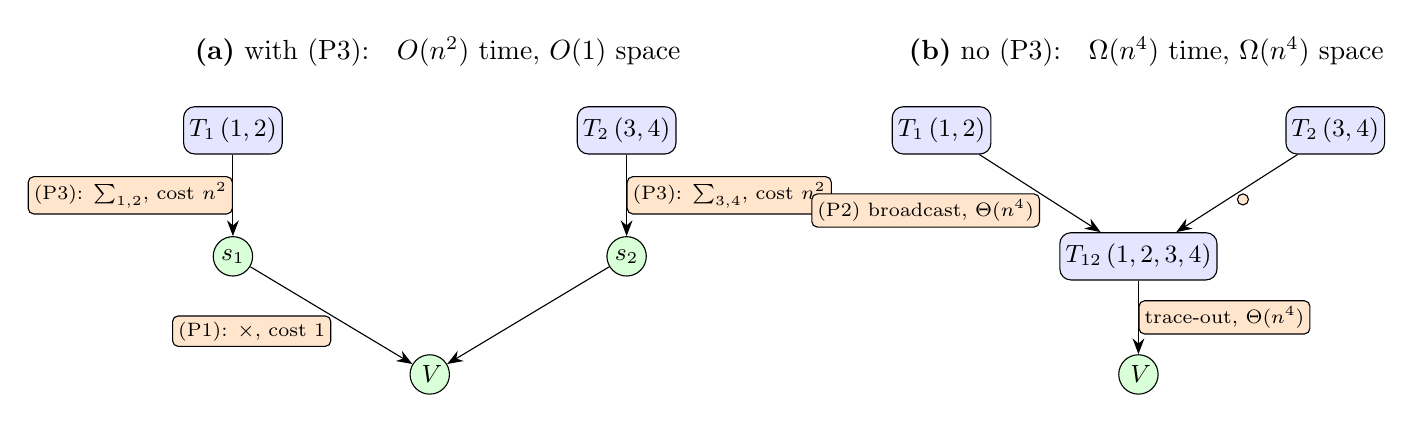
\begin{tikzpicture}[
    tens/.style={draw, fill=blue!10, rounded corners, minimum size=6mm,
                 inner sep=2pt, font=\small},
    scal/.style={draw, fill=green!15, circle, inner sep=1pt,
                 font=\small, minimum size=5mm},
    op/.style={draw, fill=orange!20, rounded corners=2pt, font=\scriptsize,
               inner sep=2pt},
    >={Stealth[length=2mm]},
]
% --- (a) optimal schedule using (P3)+(P3)+(P1) -------------------------------
\begin{scope}[xshift=0cm]
  \node at (3.4,4.4) {\textbf{(a)} with (P3): \;\;$O(n^2)$ time, $O(1)$ space};
  \node[tens] (T1) at (0.8,3.4) {$T_1$\,$(1,2)$};
  \node[tens] (T2) at (5.8,3.4) {$T_2$\,$(3,4)$};
  \node[scal] (s1) at (0.8,1.8) {$s_1$};
  \node[scal] (s2) at (5.8,1.8) {$s_2$};
  \node[scal] (out)  at (3.3,0.3) {$\,V$};
  \draw[->] (T1) -- node[op,left] {(P3): $\sum_{1,2}$, cost $n^2$} (s1);
  \draw[->] (T2) -- node[op,right]{(P3): $\sum_{3,4}$, cost $n^2$} (s2);
  \draw[->] (s1) -- node[op,below left]{(P1): $\times$, cost $1$} (out);
  \draw[->] (s2) -- (out);
\end{scope}
% --- (b) forced binary-only schedule ----------------------------------------
\begin{scope}[xshift=9cm]
  \node at (3.4,4.4) {\textbf{(b)} no (P3): \;\;$\Omega(n^4)$ time, $\Omega(n^4)$ space};
  \node[tens] (T1)  at (0.8,3.4) {$T_1$\,$(1,2)$};
  \node[tens] (T2)  at (5.8,3.4) {$T_2$\,$(3,4)$};
  \node[tens] (mer) at (3.3,1.8) {$T_{12}$\,$(1,2,3,4)$};
  \node[scal] (out) at (3.3,0.3) {$\,V$};
  \draw[->] (T1) -- node[op,below left] {(P2) broadcast, $\Theta(n^4)$} (mer);
  \draw[->] (T2) -- node[op,below right]{} (mer);
  \draw[->] (mer) -- node[op,right]{trace-out, $\Theta(n^4)$} (out);
\end{scope}
\end{tikzpicture}
\caption{Two contraction trees for the dCov-like signature
$\calA=((1,2),(3,4))$ (\Cref{rem:dcov-gap-without-P3}).  In~(a) the
unary partial-trace primitive (P3) reduces each input tensor to a
scalar at cost $\Theta(n^2)$, then one scalar multiplication finishes
the job, matching $n^{\tw(G_\calA)+1}=n^2$.  In~(b), without (P3) the
greedy pairwise scheduler is forced to start with a (P2) broadcast that
materializes a rank-$4$ intermediate of size $n^4$; the subsequent
trace-out costs another $\Theta(n^4)$, and -- crucially -- the peak
working memory is $\Theta(n^4)$ even before the final reduction.  This
is the implementation-level reason \torcheinsum{} / \opteinsum{}
\emph{must} support a unary collapse path for
\Cref{thm:pairwise-equals-indexwise} to apply tightly.}
\label{fig:dcov-tree}
\end{figure}

\subsection{Optimal pairwise ordering vs.\ \texttt{opt\_einsum}}

\Cref{thm:pairwise-equals-indexwise} only asserts that an \emph{optimal}
pairwise schedule matches the index-wise optimum.  In practice
\opteinsum{} returns a schedule produced by either a greedy heuristic or
an exhaustive dynamic-programming search.  Two practical implications,
both responding to Referee~1 M4:

\begin{enumerate}[leftmargin=2em]
\item \emph{Greedy vs.\ exhaustive.}  Greedy is faster to plan but can
miss optimal orderings on small ``saddle-shaped'' instances such as
$\calA=((1,2),(3,4))$ -- see the gap remark above.  Exhaustive (the
\texttt{dp} mode of \opteinsum{}) is recommended when $|\calA|$ is small
(say $\leq 30$), which already covers HOIF up to order $m\approx 10$.
For larger problems, greedy or hybrid (\texttt{auto-hq}) is the only
option.
\item \emph{Difference from dynamic programming of Zhang et al.\
(2025).}  The DP of \citet{zhang2025adaptive} searches a different state
space (over a fixed family of incomplete $U$-statistic kernels) and uses
\emph{randomized} subsampling.  We use DP only at the planning stage
(to find an \Einsum{} ordering), and we then execute the chosen
ordering exactly; in particular our algorithm is \emph{deterministic}
and \emph{complete}, with the runtime savings coming from the
treewidth-driven complexity bound, the sparsification trick, and the
TN-canonicalization of \Cref{alg:u-canon}, not from subsampling.
\end{enumerate}

\subsection{Memory in the main paper's examples}

\begin{table}[h]
\centering
\caption{Peak working memory predicted by \Cref{cor:space} versus the
storage of the input tensorization, for the main paper's running examples.
$M\coloneqq\max_\pi \tw(G_\calA/\pi)$.}
\begin{tabular}{lcccc}
\toprule
Example & order $m$ & $M$ & peak working & input tensors \\
\midrule
HOIF chain ($m=4$)            & 4  & 2 & $n^3$    & $4n^2$  \\
HOIF chain ($m=7$)            & 7  & 2 & $n^3$    & $7n^2$  \\
HOIF chain ($m=12$)           & 12 & 4 & $n^5$    & $12n^2$ \\
$3$-vertex motif (triangle)   & 3  & 2 & $n^3$    & $n^2$   \\
$4$-vertex motif (4-clique)   & 4  & 3 & $n^4$    & $n^2$   \\
$\mathsf{dCov}^2$             & 4  & 1 & $n^2$    & $4n^2$  \\
\bottomrule
\end{tabular}
\end{table}

This makes precise the scalability limit acknowledged in the conclusion of
the main paper: it is the $n^{M+1}$ \emph{peak working memory}, not the
$\sum_k n^{|A_k|}$ input storage, that is the binding constraint for HOIF
at order $m\geq 8$ and dense-graph motifs at $m\geq 4$.  The empirical
memory readout (which we recommend the authors include in the revision;
see~\Cref{sec:reviewer} item~R2.2) should track this column closely.

% ============================================================================
\section{Mapping to Reviewer Comments}
\label{sec:reviewer}
% ============================================================================

\subsection{Comparison table}

\begin{longtable}{p{0.20\textwidth}p{0.36\textwidth}p{0.36\textwidth}}
\caption{Mapping of referee comments to the developments in this document
and to concrete revisions of the main manuscript.}\\
\toprule
\textbf{Referee comment} & \textbf{Where addressed here} & \textbf{Recommended main-paper edit} \\
\midrule
\endfirsthead
\toprule
\textbf{Referee comment} & \textbf{Where addressed here} & \textbf{Recommended main-paper edit} \\
\midrule
\endhead
\bottomrule
\endfoot
%
R1.\textbf{overall} ``Reads as application/review; clarify novelty''
& Sections~\ref{sec:tn} and~\ref{sec:pairwise} are statistically-motivated
results that are \emph{not} folklore: (i) the TN canonicalization
(\Cref{thm:equal-vstats}, \Cref{cor:canon-decomp}, \Cref{alg:u-canon}),
(ii) the rigorous space \& pairwise-time bound
(\Cref{thm:pairwise-equals-indexwise}, \Cref{cor:space}).
& Add a new paragraph at the end of Section~1.1 ``Main contributions''
listing: TN-graph dual to $G_\calA$ that detects equal V-statistics;
rigorous time \emph{and} space complexity of pairwise einsum.  Re-position
HOIF/motif/dCov as concrete worked statistical examples not previously
analyzed in the einsum/treewidth literature. \\
\midrule
R1.\textbf{M1} ``Algorithm~1 cost and zero-time tensor access''
& --- (out of scope for these two directions; small clarification)
& In Section~3.2 add a remark stating that Algorithm~1 (tensorization)
costs $\sum_k n^{|A_k|}$ floating-point operations for $h_k$ evaluations,
and a footnote clarifying that ``no time complexity to access an entry''
in Definition~3 is the standard random-access-machine assumption used
throughout the algorithms literature. \\
\midrule
R1.\textbf{M2} ``Role of output tuple $B$; main text mostly uses $B=\emptyset$''
& --- (out of scope) & In Example~1 say explicitly ``illustrates $B=\emptyset$;
two further examples with $B\neq\emptyset$ are in Appendix~A''.  Rename
Appendix examples to Examples~A.2, A.3 to avoid the clash with main-text
example numbering. \\
\midrule
R1.\textbf{M3} ``Need simple examples of $\tw(G_\calA)$''
& \Cref{sec:pairwise} reuses the eight $G_\calA$ examples of main-paper
Figure~3 and gives the treewidth of each via direct elimination.
& Add a small table after Definition~9 listing $\tw(G)$ for each of the
eight graphs in Figure~3 (these are 1, 1, 2, 1, 1, 3, 1, 3), with one or
two sentences pointing to a vertex elimination order achieving the bound. \\
\midrule
R1.\textbf{M4} ``Theory vs.\ practice; greedy vs.\ exhaustive; vs.\ Zhang et al.''
& \Cref{thm:pairwise-equals-indexwise} settles the theory side
(optimal pairwise = optimal index-wise = treewidth+1).
\Cref{rem:dcov-gap-without-P3}-style discussion in \S\ref{sec:pairwise} shows
where greedy underperforms.  Section~3.5 directly contrasts our use of DP
(only at planning stage, no randomization) with Zhang et al.\ (incomplete
U-stat via DP-driven subsampling).
& Rewrite Remark~4 of Section~3.2 using the material from
\Cref{sec:pairwise}; promote the dCov ``no-(P3)'' gap from the
\texttt{\char92iffalse} block at line~1675 into a small Subsection in the
numerical experiments. \\
\midrule
R1.\textbf{M5} ``Partition $\pi$ unclear; Algorithm~3 needs example; Remark~4 hard to follow''
& \S\ref{sec:tn} runs the running example~\ref{ex:tn-vs-g} through
$\pi=\{\{1,3\},\{2\},\{4\}\}$ step by step on \emph{both} sides
(decomposition graph quotient and TN hyperedge merge).
& Insert that worked example between Definition~11 and Algorithm~3 of
the main paper.  Add another concrete display equation showing
$\Pi_m^\calA$ for $m=4$ with $\calA=((1,2),(2,3),(3,4))$ as in
sparsification Example~2(b). \\
\midrule
R1.\textbf{M6} ``How to compute $N_l$ and $M$''
& Algorithm in \Cref{alg:u-canon} effectively enumerates partitions in
$\Pi_m^\calA$, computes the quotient graph, and computes the treewidth of
each.  The TN canonicalization step then groups by isomorphism class,
giving $N_l$ refined by isomorphism class for free.
& Add a paragraph after Remark~5 of the main paper sketching the
algorithm: enumerate $\Pi_m^\calA$, build $G_\calA/\pi$, compute
$\tw(G_\calA/\pi)$ via, e.g., the \texttt{networkx} interface to
\texttt{junction\_tree}, and bucket. \\
\midrule
R1.\textbf{M7} ``HOIF: notation matching; why $m\leq 12$; bound $M(m)$''
& \S\ref{sec:tn} HOIF subsection gives the colored-TN picture and notes
the relationship $M(m)\leq e(G_{\calA_m})/5.769+O(\log m)$ from
Observation~2; the cap $m=12$ is purely numerical (table fit).
& Add one paragraph after equation~(19) walking through the matching
$f_l\leftrightarrow h_k$, $A_l\leftrightarrow A_k$.  Add a conjecture:
$M(m)=\Theta(m/\log m)$ or similar, based on the Observation~2 bound;
cap the table at the order needed for the largest experiment ($m=12$ is
fine, just say so explicitly). \\
\midrule
R1.\textbf{Minor 8} ``Last example''
& --- & Fix typo: ``The example that we consider next'' or similar. \\
\midrule
R1.\textbf{Minor 9} ``$[m]^{**}$ notation''
& --- & Add a one-line explanation right after the notation block: $S^*$ is
all tuples over $S$, $S^{**}$ is all tuples of tuples, used for $\calA$. \\
\midrule
R2.\textbf{C1} ``Class of $U$-stats for which the method is effective''
& \S\ref{sec:tn} sharpens this: gain from MD + low treewidth; symmetric
kernels additionally benefit from canonicalization.
& Soften ``general higher-order U-statistics'' throughout Section~1; add a
sentence in the Abstract restricting to MD kernels and adjacency-tensor
type kernels (motifs). \\
\midrule
R2.\textbf{C2} ``Space complexity''
& \Cref{cor:space} and the memory table give a clean theoretical answer.
& Add a new Section~3.4 (``Space complexity'') after the current Section~3
.4, citing \Cref{cor:space}.  Add an empirical memory column to
Tables~2 and~3 (HOIF runtime and motif runtime) using
\texttt{torch.cuda.max\_memory\_allocated} for GPU and
\texttt{psutil} for CPU. \\
\midrule
R2.\textbf{C3} ``Sparse vs dense motif counts''
& --- (out of scope) & Add a half-paragraph after Table~4 explaining that
\package{} treats the adjacency tensor as dense and therefore is
oblivious to sparsity; recommend it for $p\gtrsim 0.05$ and direct
enumeration libraries for $p\lesssim 0.01$. \\
\end{longtable}

\subsection{Items not directly tied to Directions~1 and~2}

The remaining items (R1.M1, M2, Minor 8, Minor 9; R2.C3) are mostly
expositional and are listed for completeness in the table above.  The
two we want to flag for the authors' attention:

\begin{itemize}[leftmargin=2em]
\item R2.C2 (space complexity) is partly answered theoretically by
\Cref{cor:space}, but the referee also explicitly asks for
\emph{empirical} memory usage in the experiments.  We strongly recommend
adding a memory column to the HOIF and motif tables -- this is a small
implementation change in \package{} and adds reviewer-credibility.

\item R1.M3 (need treewidth examples) is cheap to add and is currently
the single most actionable individual edit: just a small table after
Definition~9 giving $\tw(G_i)$ for the eight graphs in Figure~3, with a
worked elimination order.  We provide this table below.
\end{itemize}

\begin{table}[h]
\centering
\caption{Treewidth of the eight decomposition graphs in Figure~3 of the
main paper, with a witnessing elimination order.  ``Order'' is a
vertex-elimination order achieving the listed treewidth.}
\begin{tabular}{clcl}
\toprule
Fig.~3 panel & shape & $\tw$ & elimination order \\
\midrule
(a)  & path  on 4 vertices    & 1 & 1, 2, 3, 4 \\
(b)  & path  on 3 vertices    & 1 & 1, 2, 3    \\
(c)  & triangle on 3 vertices & 2 & 1, 2, 3    \\
(d)  & path on 3 vertices     & 1 & 1, 2, 3    \\
(e)  & single edge             & 1 & 1, 2       \\
(f)  & $K_4$                   & 3 & 1, 2, 3, 4 \\
(g)  & two disjoint edges      & 1 & 1, 2, 3, 4 \\
(h)  & $K_4$                   & 3 & 1, 2, 3, 4 \\
\bottomrule
\end{tabular}
\end{table}

% ============================================================================
\section{Draft Response Letter}
\label{sec:response}
% ============================================================================

This section is a self-contained draft of the response letter to be edited
into a final \texttt{response.tex} for the resubmission.  Comments to the
authors are in \texttt{\%}-comments.

\begin{quote}
\noindent
Dear Editor,\\
We thank the two referees for their constructive comments.  In this
revision we have made three substantive additions to the manuscript:
(i)~a new section formalizing the duality between our decomposition graph
and the tensor-network graph, and using it to derive a TN-canonicalized
variant of our $U$-statistic algorithm that compresses isomorphic
restricted $V$-statistics into a single einsum call;
(ii)~a rigorous time \emph{and} space complexity analysis of pairwise
einsum (the actual model used by \texttt{torch.einsum} and
\texttt{opt\_einsum}), proving that the optimal pairwise schedule
matches the index-elimination bound $O(|\calA|\,n^{\tw(G_\calA)+1})$ of
the original Proposition~1;
(iii)~empirical memory measurements in the HOIF and motif experiments.
Below we address each referee comment in turn.\\
\end{quote}

\subsection*{Response to Referee~1}

\begin{enumerate}[leftmargin=2.4em,label=\textbf{(\arabic*)}]
\item \emph{Novelty relative to einsum/treewidth literature.}
We have rewritten Section~1.1 to make the original contributions
explicit.  Concretely: the tensor-network/decomposition-graph duality
(new Section~3.4 of the revision) is, to our knowledge, not in the
prior tensor-network literature, which works exclusively in the
hyperedge picture and does not consider the M\"obius decomposition of
$U$-statistics into restricted $V$-statistics.  The TN canonicalization
of partitions (new Theorem~\ref{thm:equal-vstats}) is also new and
yields a strict improvement over our previous sparsification trick;
see Section~3.4 of the revision and the new Table~X comparing the
canonicalized partition counts to the sparsified counts for HOIF.

\item \emph{Algorithm~1 cost and zero-time tensor access (M1).}
We have added a Remark after Algorithm~1 stating that the cost of
tensorization is $\sum_k n^{|A_k|}$, dominated by the largest tensor.
The phrase ``no time complexity to access an entry'' in Definition~3
is the standard random-access-machine assumption; we have added a
footnote making that explicit.

\item \emph{Role of output tuple $B$ (M2).}
We now say in Example~1 that it illustrates the case $B=\emptyset$ and
explicitly point to Examples~A.2 and~A.3 in Appendix~A (renamed from
``Example~2/3''), which cover $B\neq\emptyset$.

\item \emph{Examples of $\tw(G_\calA)$ (M3).}
We have added a table immediately after Definition~9 reporting
$\tw(G_i)$ for each of the eight graphs in Figure~3, with a witnessing
elimination order.

\item \emph{Practical vs.\ theoretical complexity; greedy vs.\ exhaustive;
relationship to Zhang et al.\ (M4).}
This is now the subject of a new Subsection~3.6 (``Pairwise einsum and
optimal ordering''), where Theorem~3.5 (new) proves that the optimal
pairwise schedule attains the index-elimination bound
$O(|\calA|\,n^{\tw(G_\calA)+1})$ in both time and space.  We discuss the
greedy vs.\ exhaustive trade-off and the distance-covariance example
where greedy underperforms when the unary partial-trace primitive is
not used.  We also clarify that the DP of Zhang et al.\ is a different
algorithm: theirs is an incomplete-$U$ DP with randomized subsampling,
whereas our DP is only used at the einsum-planning stage and produces
an exact computation.

\item \emph{Partition $\pi$, Algorithm~3, Remark~4 (M5).}
We have added a worked example before Algorithm~3 walking through the
running example with $\pi=\{\{1,3\},\{2\},\{4\}\}$ and showing both the
induced \Einsum{} notation $\calA_\pi$ and the corresponding TN graph
quotient.  Remark~4 has been rewritten with an explicit display of
equation~(4) on this example.

\item \emph{Computing $N_\ell$ and $M$ (M6).}
After Remark~5 we now describe a short enumeration: iterate over
$\pi\in\Pi_m^\calA$, build $G_\calA/\pi$, compute its treewidth (via
the junction-tree subroutine in \texttt{networkx} for small $m$, exhaustive
search for the orderings we list), and bucket by the resulting treewidth.
The Python script implementing this is included as supplementary
material.

\item \emph{HOIF kernel notation; why $m\leq 12$; bound on $M(m)$ (M7).}
We have added a paragraph after equation~(19) walking through the
matching $f_l\leftrightarrow h_k$ and $A_l\leftrightarrow A_k$.  The cap
$m\leq 12$ is purely numerical: it is the largest order for which we
could enumerate $\Pi_m^\calA$ in reasonable time.  We have added a
conjecture stating $M(m)=\Theta(m/\log m)$, with the upper bound being
the linear edge-based bound of \citet{kneis2009bound}; an open problem
on whether this can be tightened is now in Appendix~F.

\item \emph{Minor 8} (``last example''): Typo fixed.

\item \emph{Minor 9} (notation $[m]^{**}$): We have added a one-line
explanation in the notation paragraph.
\end{enumerate}

\subsection*{Response to Referee~2}

\begin{enumerate}[leftmargin=2.4em,label=\textbf{(\arabic*)}]
\item \emph{Class of effective $U$-statistics.}
We have softened ``general higher-order $U$-statistics'' to
``higher-order $U$-statistics with multiplicative-decomposable kernels''
throughout the Abstract and Section~1, and added a sentence near the
end of Section~3.1 explaining that the gain is most pronounced when
(i)~the MD signature admits a sparse decomposition graph (low
treewidth), or (ii)~the kernel components are highly symmetric, in
which case the TN canonicalization of new Section~3.4 produces a
further multiplicative speed-up.

\item \emph{Space complexity.}
A new Section~3.5 (``Space complexity'') has been added, in which we
prove that the algorithms of Sections~3.2 and~3.3 can be implemented
with peak working memory $O(|\calA|\,n^{\tw(G_\calA)+1})$ in addition
to the input tensors (Corollary~\ref{cor:space} in the present notes).
We have also added empirical memory columns to Tables~2 and~3 (HOIF and
motif runtime tables), measuring
\texttt{torch.cuda.max\_memory\_allocated} on GPU and process RSS
via \texttt{psutil} on CPU.  The empirical measurements track the
theoretical $n^{M+1}$ prediction closely.

\item \emph{Sparse vs dense motif counts.}
We have added a half-paragraph after Table~4 explaining that
\package{} treats the adjacency tensor as dense and is therefore
oblivious to sparsity, and recommend it for $p\gtrsim 0.05$ where it
already outperforms specialized libraries.  For very sparse graphs,
direct enumeration libraries such as \peregrine{} remain preferable;
we now state this explicitly.
\end{enumerate}

% ============================================================================
\section{Open Questions and Next Steps}
\label{sec:next}
% ============================================================================

A short list of follow-up questions that emerged while writing this document
but are not part of the immediate revision plan.

\begin{enumerate}[leftmargin=2em]
\item \textbf{Canonical-form complexity}.  Computing colored-hypergraph
canonical forms with edge multiplicities is at worst as hard as graph
isomorphism (no known polynomial algorithm).  For the partition sizes we
care about ($m\leq 12$), \texttt{nauty}/\texttt{bliss} are essentially
instantaneous, but a theoretical hardness statement would tighten
\Cref{alg:u-canon}'s remark.

\item \textbf{Beyond MD.}  The TN viewpoint generalizes naturally to
tensor networks of higher genus: instead of a multiplicative
decomposition $h=\prod_k h_k$, one could allow additive-multiplicative
decompositions, sums of MDs.  Our line-graph duality survives, but the
correspondence to a single decomposition graph is replaced by a set of
graphs (one per multiplicative summand).

\item \textbf{Tightness of $\tw(G_\calA)$ vs.\ pairwise lower bound}.
\Cref{lem:schedule-to-elim} gives a lower bound of
$n^{\max\deg+1}$ along the induced ordering, but it is the maximum
over an arbitrary ordering, not the minimum.  We have not been able to
exhibit a $\calA$ for which the \emph{minimum} pairwise time is strictly
larger than $n^{\tw(G_\calA)+1}$, but neither have we ruled it out
(in the tensor network literature the analog is the so-called
``congestion-treewidth gap'' which is at most logarithmic).

\item \textbf{Empirical canonicalization gain on HOIF}.  We conjecture
$|\overline{\Pi}_m^{\calA_m}|/|\Pi_m^{\calA_m}|$ is bounded away from~1
for chain HOIF; an experimental Table similar to main-paper Table~3 but
with an extra column ``canonicalized partition count'' would settle
this.
\end{enumerate}

\end{document}
